\subsubsection{Caso d’uso UC8.1.3.5: Creazione domanda a ordinamento di immagini}
\label{UC8.1}
	\begin{figure}[h]
		\centering
			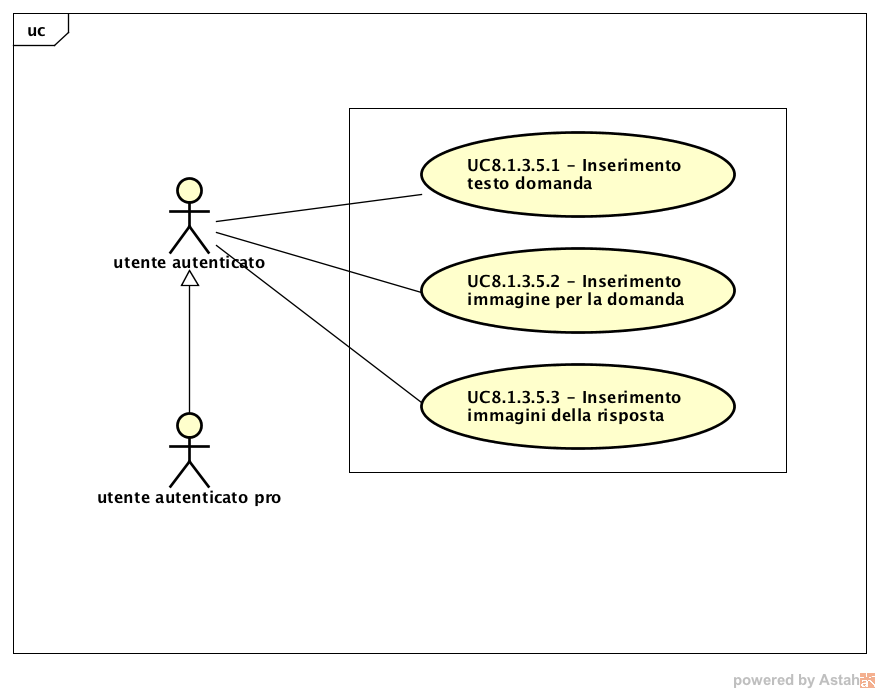
\includegraphics[scale=0.45,keepaspectratio]{UML/UC8_1_3_5.png}
		\caption{UC8.1.3.5: Creazione domanda a ordinamento immagini}
	\end{figure}
\begin{itemize}
	\item\textbf{Attori}: utente autenticato, utente autenticato pro;
	\item\textbf{Scopo e descrizione}: gli attori possono inserire una domanda del tipo ordinamento di immagini;
	\item\textbf{Precondizione}: il sistema mostra agli attori il form di inserimento dei campi dati per la tipologia di domanda scelta; 
	\item \textbf{Postcondizione}: gli attori hanno inserito tutti i campi dati obbligatori;
	\item\textbf{Scenario principale}: gli attori possono inserire i seguenti dati:
	\begin{itemize}
		\item Gli attori devono compilare il campo dati destinato alla scrittura del testo della domanda (UC8.1.3.5.1);
		\item Gli attori inseriscono un'immagine per il testo della domanda (UC8.1.3.5.2)
		\item Gli attori devono inserire le immagini nel giusto ordine (UC8.1.3.5.3);
	\end{itemize}
\end{itemize}

\subsubsection{Caso d’uso UC8.1.3.5.1: Inserimento testo domanda}
\begin{itemize}
	\item\textbf{Attori}: utente autenticato, utente autenticato pro;
	\item\textbf{Scopo e descrizione}: lo scopo di questa funzionalità è offrire agli attori la possibilità di inserire il testo della domanda;
	\item\textbf{Precondizione}: gli attori hanno scelto la modalità di creazione della domanda a ordinamento di immagini; 
	\item \textbf{Postcondizione}: gli attori hanno inserito il testo della domanda;
	\item\textbf{Scenario principale}: gli attori devono inserire il testo della domanda. 
\end{itemize}

\subsubsection{Caso d’uso UC8.1.3.5.2: Inserimento immagine per testo domanda}
\begin{itemize}
	\item\textbf{Attori}: utente autenticato, utente autenticato pro;
	\item\textbf{Scopo e descrizione}: lo scopo di questa funzionalità è offrire agli attori la possibilità di inserire un'immagine relativa domanda;
	\item\textbf{Precondizione}: gli attori hanno scelto la modalità di creazione della domanda a ordinamento di immagini; 
	\item \textbf{Postcondizione}: gli attori hanno inserito un'immagine relativa alla domanda;
	\item\textbf{Scenario principale}: gli attori inseriscono un'immagine relativa alla domanda. 
\end{itemize}

\subsubsection{Caso d’uso UC8.1.3.5.3: Inserimento immagini della risposta}
\begin{itemize}
	\item\textbf{Attori}: utente autenticato, utente autenticato pro;
	\item\textbf{Scopo e descrizione}: lo scopo di questa funzionalità è offrire agli attori la possibilità di inserire le immagini per la risposta della relativa domanda;
	\item\textbf{Precondizione}: gli attori hanno scelto la modalità di creazione della domanda a ordinamento di immagini; 
	\item \textbf{Postcondizione}: gli attori hanno inserito delle immagini in ordine corretto per la relativa alla domanda;
	\item\textbf{Scenario principale}: gli attori inseriscono delle immagini in ordine corretto per la relativa domanda. 
\end{itemize}